
\blueheader
\begin{frame}{2B: Nedre trappesum til en ikke er strengt voksende funksjon}
Merk at generelt tar 
\begin{itemize}
    \item nedre trappesum utgangspunkt i den minste høyden til rektanglet.\\
    \item og øvre trappesum tar utgangspunkt i den største høyden til rektanglet.
\end{itemize}
\begin{figure}
    \centering
    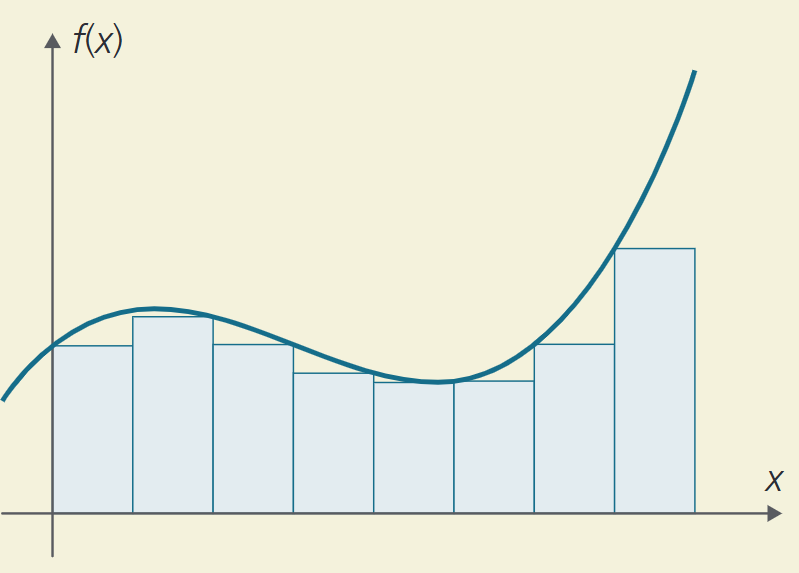
\includegraphics[width=0.6\linewidth]{R2-K2A-17.png}
\end{figure}
\end{frame}


\blueheader
\begin{frame}{2B: Venstre- og høyre-tilnærming}
\begin{figure}
    \centering
    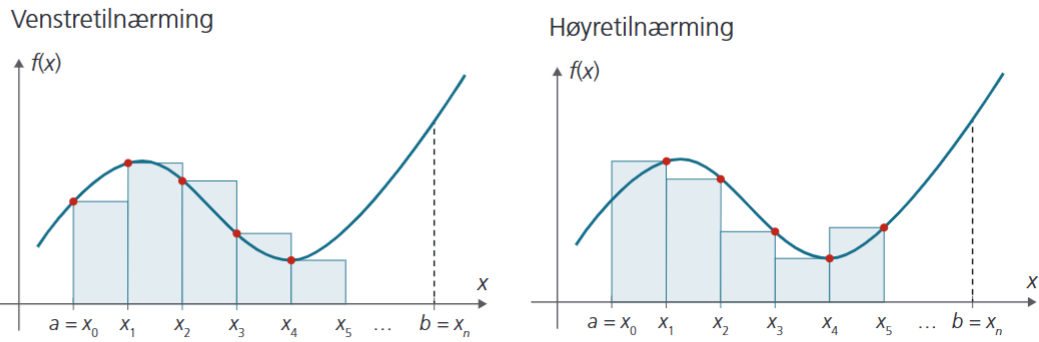
\includegraphics[width=\linewidth]{R2-K2B-2.png}
\end{figure}
\end{frame}

\blueheader
\begin{frame}{2B: Riemannsummer. Velger en vilkårlig x-verdi, $x^*\in[x_{i-1},x_i]$}
    \begin{columns} 
        \begin{column}{0.35\textwidth}
    \textbf{Venstretilnærming:}
        \begin{equation*}
            \sum_{i=1}^n f(x_{i-1})\cdot \Delta x
        \end{equation*}
      \textbf{Høyretilnærming:}
        \begin{equation*}
            \sum_{i=1}^n f(x_{i})\cdot \Delta x
        \end{equation*}
    \textbf{Riemansum:}
       \begin{equation*}
            \sum_{i=1}^n f(x^*_{i})\cdot \Delta x
        \end{equation*}
        \end{column}
        \begin{column}{0.65\textwidth}
            \centering
            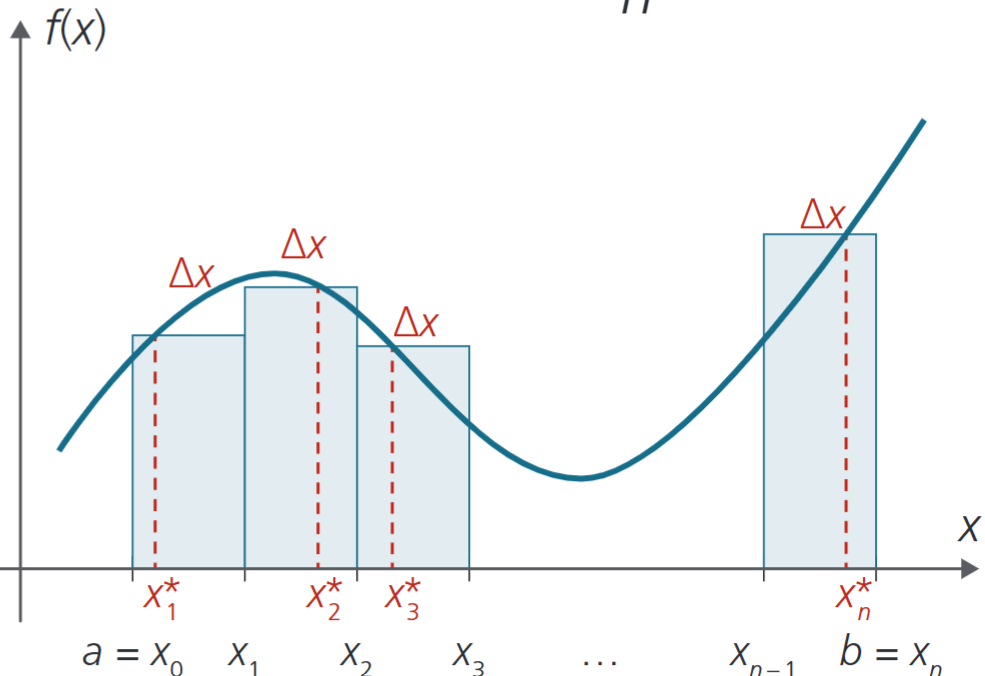
\includegraphics[width=1\linewidth]{R2-K2B-1.png}
        \end{column}
    \end{columns}
\end{frame}

\redheader
\begin{frame}{2B: Det bestemte integralet}
    Det bestemte integralet kan uttrykkes som en grenseverdi til en følge av riemannsummer.

    \begin{equation*}
        \int_a^b f(x)\;dx=\lim_{n\rightarrow\infty}\sum_{i=1}^nf(x_i^*)\cdot \Delta x, \:\;\; \text{der} \;\;\; \Delta x = \frac{b-a}{n}
    \end{equation*}
\end{frame}

\redheader
\begin{frame}{2B: Rektangelmetoden med venstretilnærming}
 \begin{equation*}
        \int_a^b f(x)\;dx=\lim_{n\rightarrow\infty}\sum_{i=1}^nf(x_{i-1})\cdot \Delta x, \:\;\; \text{der} \;\;\; x_{i-1}=a+(i-1)\cdot \Delta x
    \end{equation*}
    \begin{figure}
        \centering
   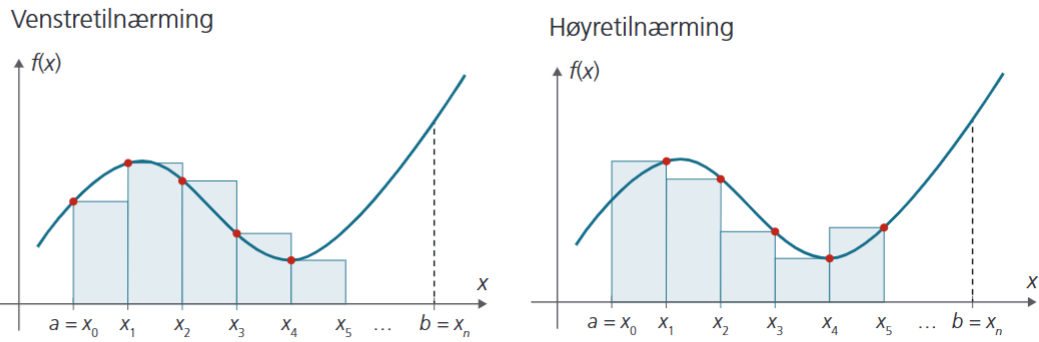
\includegraphics[width=\linewidth]{R2-K2B-2.png}
    \end{figure}
\end{frame}

\redheader
\begin{frame}{2B: Rektangelmetoden med høyretilnærming}
 \begin{equation*}
        \int_a^b f(x)\;dx=\lim_{n\rightarrow\infty}\sum_{i=1}^nf(x_{i})\cdot \Delta x, \:\;\; \text{der} \;\;\; x_{i}=a+i\cdot \Delta x
    \end{equation*}

     \begin{figure}
        \centering
   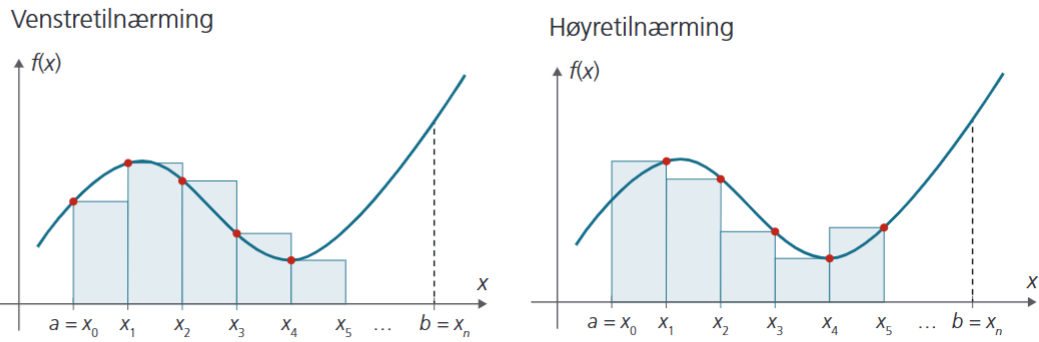
\includegraphics[width=\linewidth]{R2-K2B-2.png}
    \end{figure}
\end{frame}


\greenheader
\begin{frame}{2B: Eksempel 5 side 106 (Venstretilnærming)}
\begin{figure}
    \centering
    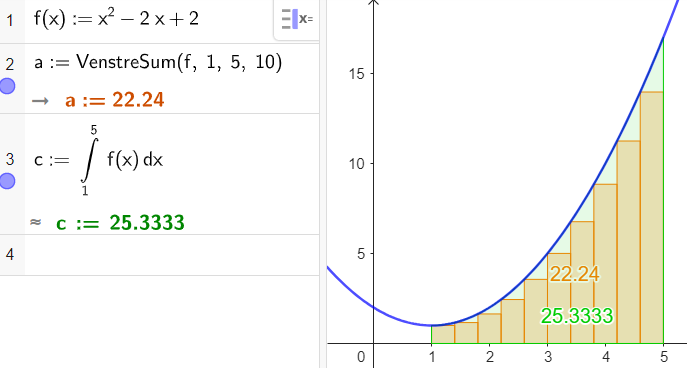
\includegraphics[width=\linewidth]{R2-K2B-3.png}
\end{figure}
\end{frame}

\greenheader
\begin{frame}[fragile]{2B: Eksempel 5 side 106: Venstretilnærming og høyretilnærming i python}
\begin{minted}[fontsize=\small]{python}
a, b = 1, 5               # Nedre og øvre grense i intervallet [a, b]
n = 10                    # Antall rektangler

def f(x):
  return x**2 - 2*x + 2

venstre_sum = 0           # Summen av arealene til venstre-tilnærming-rektangler
høyre_sum   = 0           # Summen av arealene til høyre-tilnærming-rektangler
delta_x = (b-a)/n         # Rektangelbredden

for i in range(1, n+1):
  venstre_sum = venstre_sum + f(a+(i-1)*delta_x)*delta_x
  høyre_sum = høyre_sum + f(a+i*delta_x)*delta_x

print(f"Venstresummen: {round(venstre_sum,2)}")     # Venstresummen: 22.24
print(f"Høyresummen: {round(høyre_sum,2)}")         # Høyresummen: 28.64
print(f"Gjennomsnitt: {(venstre_sum+høyre_sum)/2}") # Gjennomsnitt: 25.44
\end{minted}
\end{frame}

\greenheader
\begin{frame}{2B: Eksempel 6 side 108: Venstretilnærming}
Funksjonen $f$ har verditabellen
\begin{table}[h]
\centering
\begin{tabular}{c|ccccccccc}
$x$ & 0 & 0,5 & 1 & 1,5 & 2 & 2,5 & 3 & 3,5 & 4 \\
\hline
$f(x)$ & 13,1 & 16,3 & 0 & 8,2 & 19,7 & 24,8 & 28,1 & 27,3 & 21,0 \\
\end{tabular}
\end{table}
Lag et program som finner en tilnærmingsverdi for $\int_0^4 f(x)\;dx$ med en venstretilnærming.
\begin{figure}
    \centering
    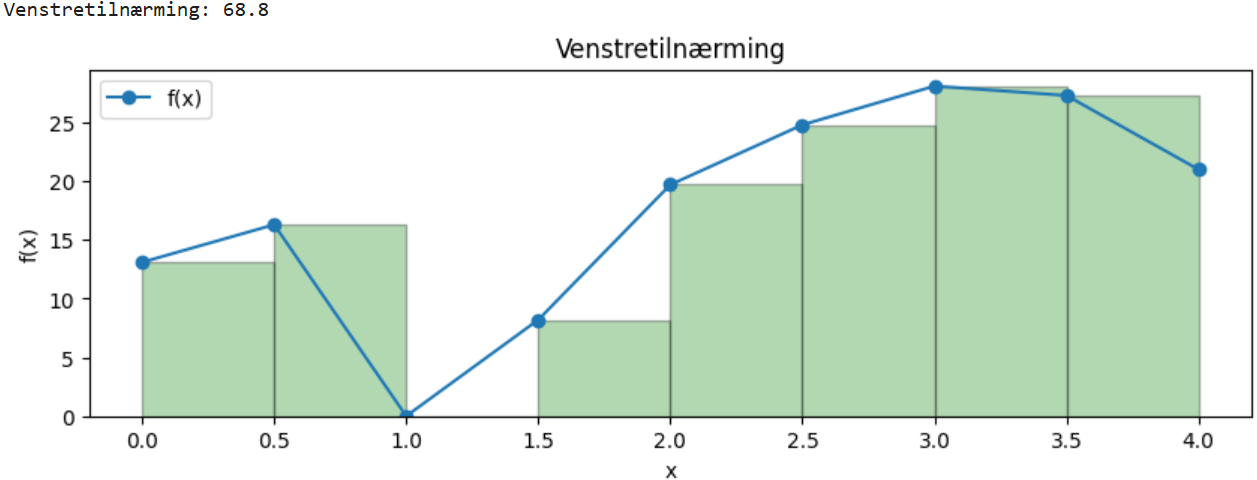
\includegraphics[width=0.9\linewidth]{R2-K2B-4.png}

\end{figure}
\end{frame}

\greenheader
\begin{frame}[fragile]{2B: Eksempel 6 side 108: Venstretilnærming}
\begin{minted}[fontsize=\small]{python}
# lister med x-verdier og funksjonsverdier
x = [0, 0.5, 1, 1.5, 2, 2.5, 3, 3.5, 4]
f = [13.1, 16.3, 0, 8.2, 19.7, 24.8, 28.1, 27.3, 21.0]

delta_x = x[1] - x[0]     # rektangelbredde
n = len(x)                # antall x-verdier i lista
summen = 0

# Legg merke til at n = len(x) = 9, og siden "i" i for-løkken 
# starter på 0, må "i" gå til n-1=8, og at maks verdi for "i" er 7.

for i in range(n-1):    
  summen = summen + f[i] * delta_x

print(round(summen, 1)) # Output: 68.8

# Legg merke til at det står f[i], og ikke f[i-1], selv om dette er en 
# venstretilnærming. Det er fordi "i" i for-løkken starter på null. 
\end{minted}
\end{frame}




\redheader
\begin{frame}{2B: Midtpunkttilnærming}
 \begin{equation*}
        \int_a^b f(x)\;dx\approx\sum_{i=1}^nf(m_{i})\cdot \Delta x, \:\;\; \text{der} \;\;\; m_{i}=a+\left(i-\frac{1}{2}\right)\cdot \Delta x
    \end{equation*}

     \begin{figure}
        \centering
   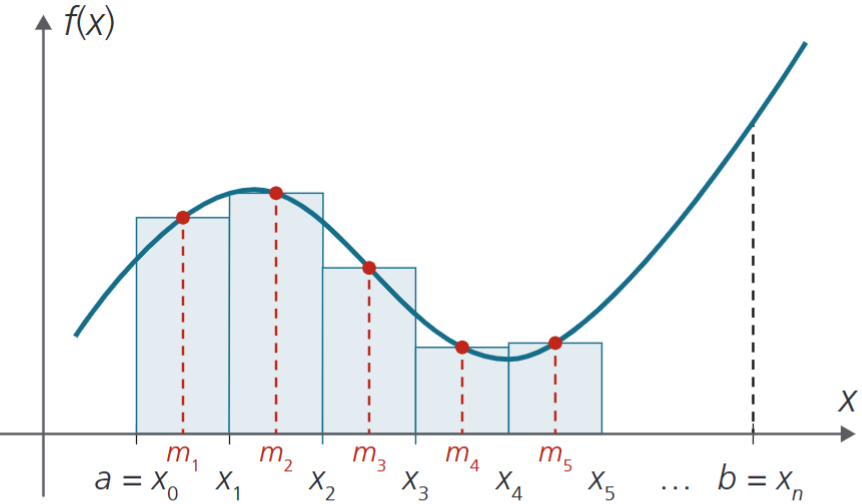
\includegraphics[width=0.7\linewidth]{R2-K2B-5.png}
    \end{figure}
\end{frame}


\greenheader
\begin{frame}{2B: Eksempel 5 side 105: Midtpunkttilnærming. Fasit: 25,33}
Funksjonen $f$ er gitt ved $f(x)=x^2-2x+2$. Lag et program som finner en tilnærmingsverdi for integralet ved å bruke midtpunkttilnærming med 10 kvadrater.
\[
\int_1^5f(x)\;dx
\].
\begin{figure}
    \centering
    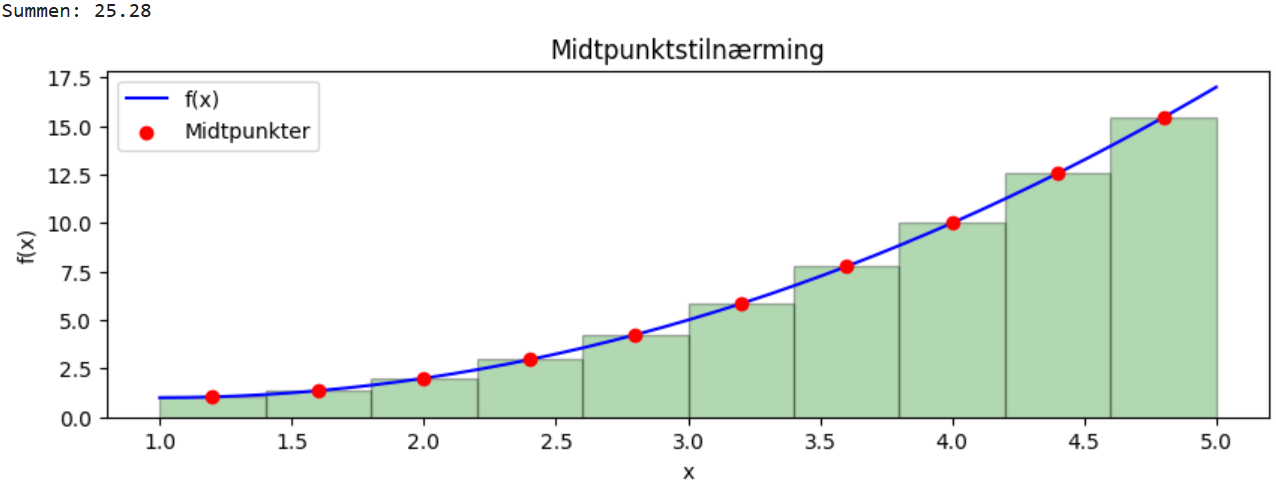
\includegraphics[width=0.9\linewidth]{R2-K2B-7.png}
\end{figure}
\end{frame}


\greenheader
\begin{frame}[fragile]{2B: Eksempel 5 side 105: Midtpunkttilnærming. Fasit: 25,33}
\begin{minted}[fontsize=\small]{python}
a, b = 1, 5     # Nedre og øvre grense i intervallet [a, b]
n = 10          # Antall rektangler

def f(x):
    return x**2 - 2*x + 2

delta_x = (b - a) / n
summen = 0.0

for i in range(n):
    x_midt = a + (i + 0.5) * delta_x
    summen = summen + f(x_midt) * delta_x

print(f"Midtpunktsummen: {round(summen, 2)}") # Output: 25.28
\end{minted}
\end{frame}

\greenheader
\begin{frame}{2B: Eksempel 6 side 108: Midtpunkttilnærming}
Funksjonen $f$ har verditabellen
\begin{table}[h]
\centering
\begin{tabular}{c|ccccccccc}
$x$ & 0 & 0,5 & 1 & 1,5 & 2 & 2,5 & 3 & 3,5 & 4 \\
\hline
$f(x)$ & 13,1 & 16,3 & 0 & 8,2 & 19,7 & 24,8 & 28,1 & 27,3 & 21,0 \\
\end{tabular}
\end{table}
Lag et program som finner en tilnærmingsverdi for $\int_0^4 f(x)\;dx$ med en midtpunkttilnærming.
\begin{figure}
    \centering
    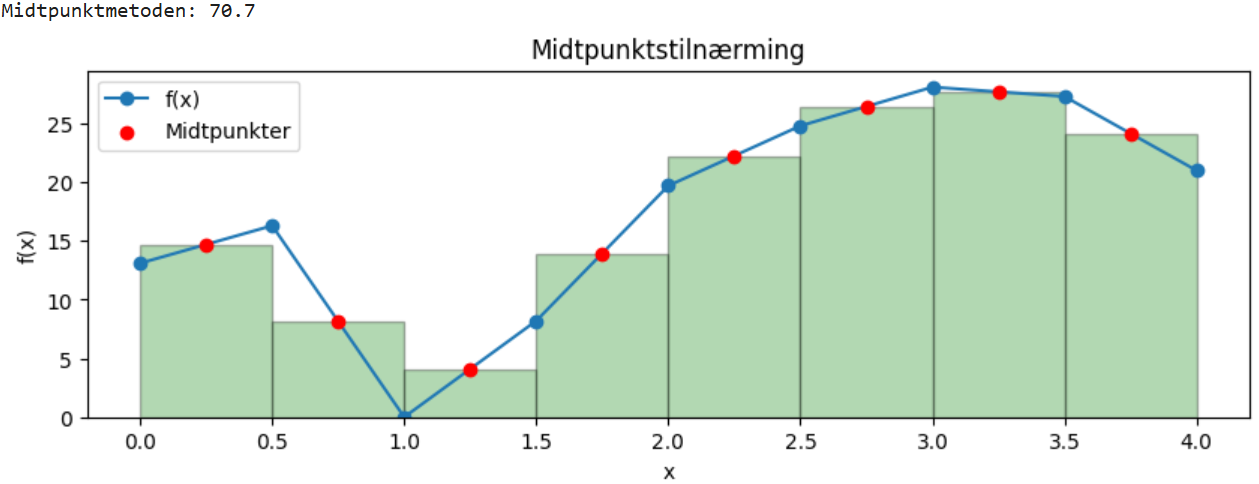
\includegraphics[width=0.8\linewidth]{R2-K2B-6.png}

\end{figure}
\end{frame}

\greenheader
\begin{frame}[fragile]{2B: Eksempel 6 side 108: Midtpunkttilnærming}
\begin{minted}[fontsize=\small]{python}
# To lister med x-verdier og funksjonsverdier
x = [0, 0.5, 1, 1.5, 2, 2.5, 3, 3.5, 4]
f = [13.1, 16.3, 0, 8.2, 19.7, 24.8, 28.1, 27.3, 21.0]

delta_x = x[1] - x[0]  # rektangelbredde
n = len(x)  # antall x-verdier i lista
summen = 0

# Midtpunktstilnærming
for i in range(n-1):
    # Bruk gjennomsnittet som approksimasjon av funksjonsverdi i midten
    midt_f = (f[i] + f[i+1]) / 2
    summen = summen + midt_f * delta_x

print(round(summen, 1))

\end{minted}
\end{frame}


\blueheader
\begin{frame}{2B: Arealformelen til et trapes}
\begin{columns}[c] % [c] = midtstill innholdet vertikalt
  \begin{column}{0.45\textwidth}
    \[
      A = \frac{h}{2}(a+b)
    \]
    \begin{itemize}
      \item \(a, b\) = parallelle sider
      \item \(h\) = høyden
    \end{itemize}

Men i vårt tilfelle er det bedre å skrive arealformelen slik:

\begin{equation*}
    A=\frac{4-2}{2}\left(f(2)+f(4)\right)
\end{equation*}

Generelt får vi (hvis \emph{i} starter på 1):
\begin{equation*}
    A=\frac{\Delta x}{2}\left(f(x_{i-1})+f(x_{i})\right)
\end{equation*}
  \end{column}
  \begin{column}{0.55\textwidth}
    \begin{figure}
      \centering
      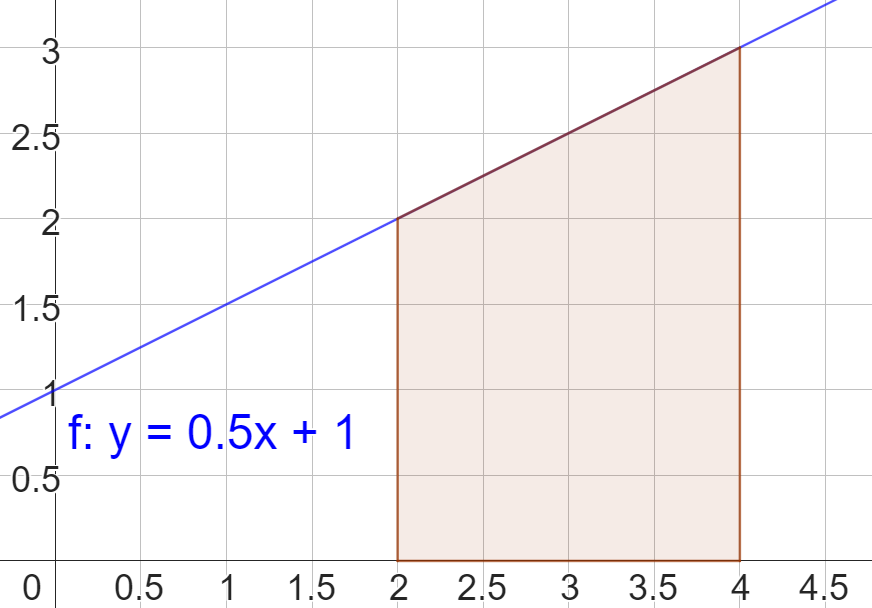
\includegraphics[width=\linewidth]{R2-K2B-8.png}
    \end{figure}
  \end{column}
\end{columns}
\end{frame}

\redheader
\begin{frame}{2B: Trapesetoden}
 \begin{equation*}
        \int_a^b f(x)\;dx\approx\frac{\Delta x}{2}\left(f(a)+f(b)+2\cdot \sum_{i=1}^{n-1}f(x_i)\right),\;\;\;\texttt{der}\;\;\; x_i=a+i\cdot \Delta x
    \end{equation*}
     \begin{figure}
        \centering
   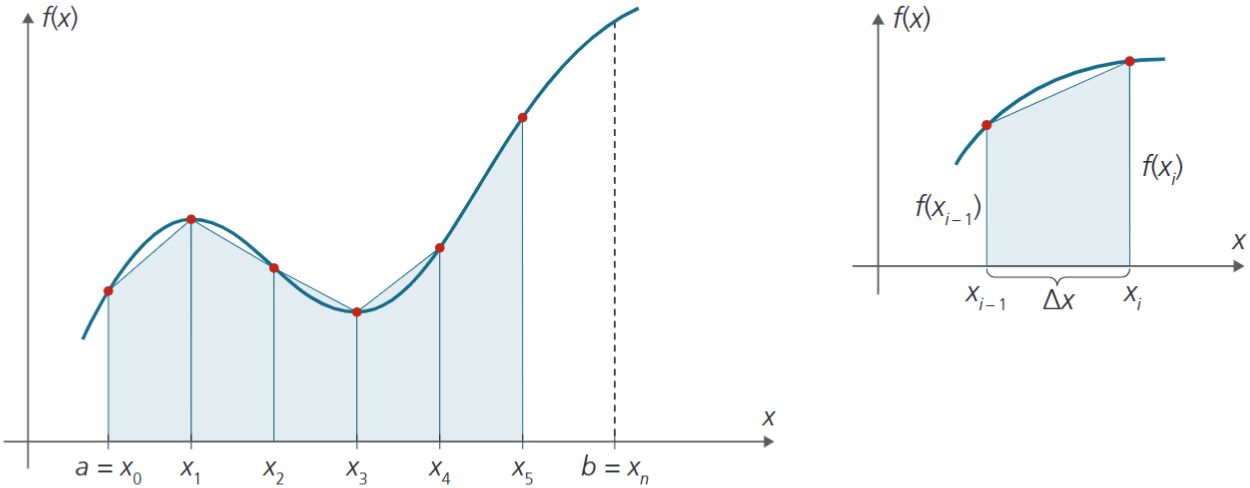
\includegraphics[width=0.8\linewidth]{R2-K2B-9.png}
    \end{figure}
(Beviset står på side 110)
\end{frame}


\greenheader
\begin{frame}{2B: Eksempel 5 side 105: Trapesmetoden. Fasit: 25,33}
Funksjonen $f$ er gitt ved $f(x)=x^2-2x+2$. Lag et program som finner en tilnærmingsverdi for integralet ved å bruke trapesmetoden med 10 kvadrater.
\[
\int_1^5f(x)\;dx
\].
\begin{figure}
    \centering
    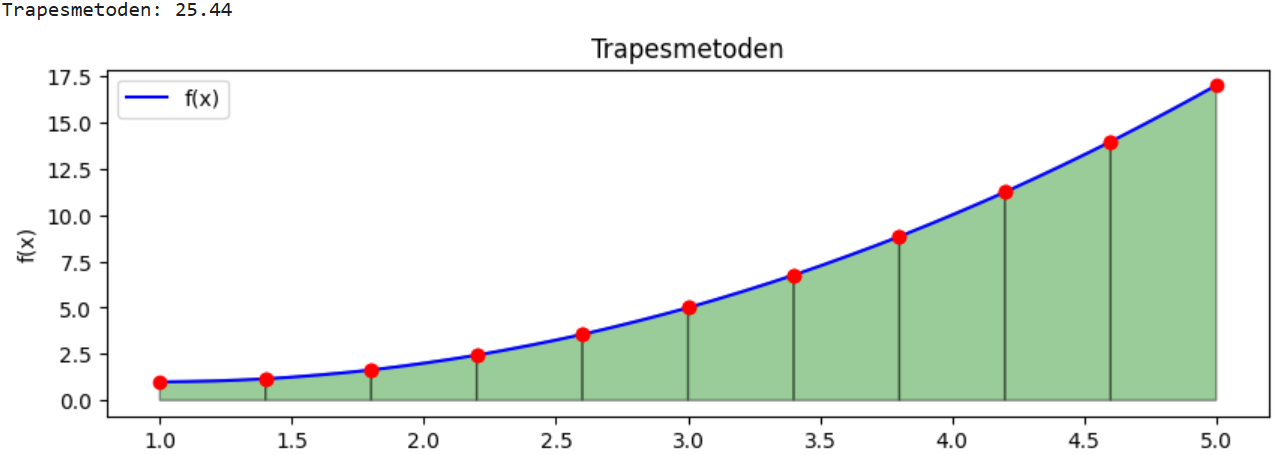
\includegraphics[width=0.9\linewidth]{R2-K2B-10.png}
\end{figure}
\end{frame}


\greenheader
\begin{frame}[fragile]{2B: Eksempel 5 side 105: Trapesmetoden. Fasit: 25,33}
\begin{minted}[fontsize=\small]{python}
a, b = 1, 5   # Intervallet [a, b]
n = 10        # Antall delintervaller
delta_x = (b - a) / n
summen = 0.0

def f(x):
    return x**2 - 2*x + 2

# Bruker List comprehension til å lage lister med x- og y-verdier. 
x_liste = [a + i*delta_x for i in range(n+1)]
y_liste = [f(x) for x in x_liste]

# Trapesmetoden. Utfordring: Forklar at denne koden 
# stemmer med trapes-metode-formelen.
for i in range(n): 
    summen = summen + (y_liste[i] + y_liste[i+1]) * delta_x / 2

print(f"Trapesmetoden: {round(summen, 2)}") # Output: 25.44
\end{minted}
\end{frame}


\greenheader
\begin{frame}{2B: Eksempel 6 side 108: Trapesmetoden}
Funksjonen $f$ har verditabellen
\begin{table}[h]
\centering
\begin{tabular}{c|ccccccccc}
$x$ & 0 & 0,5 & 1 & 1,5 & 2 & 2,5 & 3 & 3,5 & 4 \\
\hline
$f(x)$ & 13,1 & 16,3 & 0 & 8,2 & 19,7 & 24,8 & 28,1 & 27,3 & 21,0 \\
\end{tabular}
\end{table}
Lag et program som finner en tilnærmingsverdi for $\int_0^4 f(x)\;dx$ med en trapesmetoden.
\begin{figure}
    \centering
    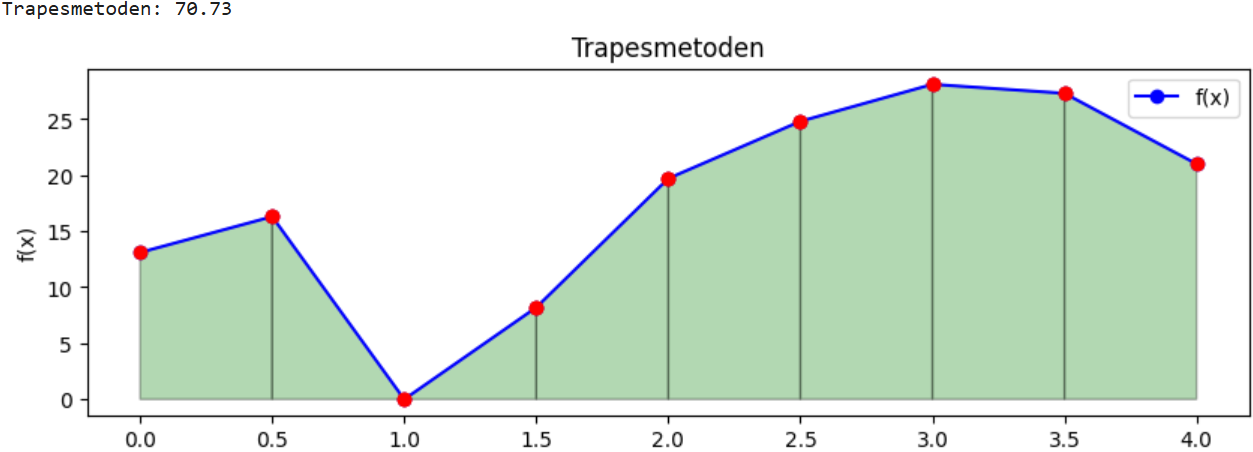
\includegraphics[width=0.8\linewidth]{R2-K2B-11.png}

\end{figure}
\end{frame}

\greenheader
\begin{frame}[fragile]{2B: Eksempel 6 side 108: Trapesmetoden}
\begin{minted}[fontsize=\normalsize]{python}
# Dataene fra tabellen
x = [0, 0.5, 1, 1.5, 2, 2.5, 3, 3.5, 4]
f = [13.1, 16.3, 0, 8.2, 19.7, 24.8, 28.1, 27.3, 21.0]

delta_x = x[1] - x[0]  # bredde
n = len(x) - 1         # antall delintervaller
summen = 0

# Trapesmetoden
for i in range(n):
    summen += (f[i] + f[i+1]) * delta_x / 2

print(f"Trapesmetoden: {round(summen, 2)}") # Output: 70.73
\end{minted}
\end{frame}






















% -----------------------
\greenheader
\begin{frame}[fragile]{2B: Generell pythonkode for å regne ut nedre trappesum  (Utfordring)}
\begin{minted}[fontsize=\small]{python} 
def f(x):
    return 0.1*x*(x-4)*(x-8)  # Funksjonen vi skal integrere tilnærmet

start, slutt = 0, 8           # Integrasjonsintervall [0, 8]
bredde = 0.1                  # Bredde på hvert rektangel
antall = round((slutt-start)/bredde)  # Antall rektangler i intervallet
N, Ø = 0, 0  # Startverdier for nedre og øvre trappesum

for i in range(antall):
    x_venstre = start + i*bredde      # Venstre endepunkt for intervallet
    x_høyre = x_venstre + bredde      # Høyre endepunkt for intervallet
    f_venstre = f(x_venstre)          # Funksjonsverdi i venstre endepunkt
    f_høyre = f(x_høyre)              # Funksjonsverdi i høyre endepunkt
    N = N + bredde * min(f_venstre, f_høyre)  # Areal med minste funksjonsverdi
    
print(f"Antall rektangler: {antall}") 
print(f"Rektangelbredde: {bredde}")
print(f"Nedre trappesum: {N}")
\end{minted}
\end{frame}


\greenheader
\begin{frame}[fragile]{2B: Generell pythonkode for å regne ut øvre trappesum  (Utfordring) }
\begin{minted}[fontsize=\small]{python}
def f(x):
    return 0.1*x*(x-4)*(x-8)  # Funksjonen vi skal integrere tilnærmet

start, slutt = 0, 8           # Integrasjonsintervall [0, 8]
bredde = 0.1                  # Bredde på hvert rektangel
antall = round((slutt-start)/bredde)  # Antall rektangler i intervallet
N, Ø = 0, 0  # Startverdier for nedre og øvre trappesum

for i in range(antall):
    x_venstre = start + i*bredde      # Venstre endepunkt for intervallet
    x_høyre = x_venstre + bredde      # Høyre endepunkt for intervallet
    f_venstre = f(x_venstre)          # Funksjonsverdi i venstre endepunkt
    f_høyre = f(x_høyre)              # Funksjonsverdi i høyre endepunkt
    Ø = Ø + bredde * max(f_venstre, f_høyre)  # Areal med største funksjonsverdi

print(f"Antall rektangler: {antall}") 
print(f"Rektangelbredde: {bredde}")
print(f"Øvre trappesum: {Ø}")
\end{minted}
\end{frame}